\documentclass{article}
\textheight 23.5cm \textwidth 15.8cm
%\leftskip -1cm
\topmargin -1.5cm \oddsidemargin 0.3cm \evensidemargin -0.3cm
%\documentclass[final]{siamltex}

\usepackage{verbatim}
\usepackage{fancyhdr}
\usepackage{amssymb,ctex}
\usepackage{mathrsfs}
\usepackage{latexsym,amsmath,amssymb,amsfonts,epsfig,graphicx,cite,psfrag}
\usepackage{eepic,color,colordvi,amscd}
\usepackage{enumerate}
\usepackage{enumitem}
\usepackage{booktabs}
\usepackage{graphicx}
\usepackage{float}
\usepackage{wrapfig}
\usepackage{multirow}
\usepackage{subfigure}
\usepackage{diagbox}


\title{USTC\_CG HW2 Image Warping}
\author{张继耀,PB20000204}

\begin{document}
	\maketitle
	
	\tableofcontents
	
	\section {问题介绍}
	\subsection{主要目的}
	
	\begin{itemize}
		\item 阅读论文,实现IDW、RBF算法
	\end{itemize}

	\begin{itemize}
		\item 进行内存泄露检测
	\end{itemize}

	\begin{itemize}
		\item 填补可能产生的白缝
	\end{itemize}

	
	\section{算法设计}
	
	\subsection{程序框架}
	
	下面我们首先给出整个项目的类视图
	
		\begin{figure}[H]
		\begin{center}
			
			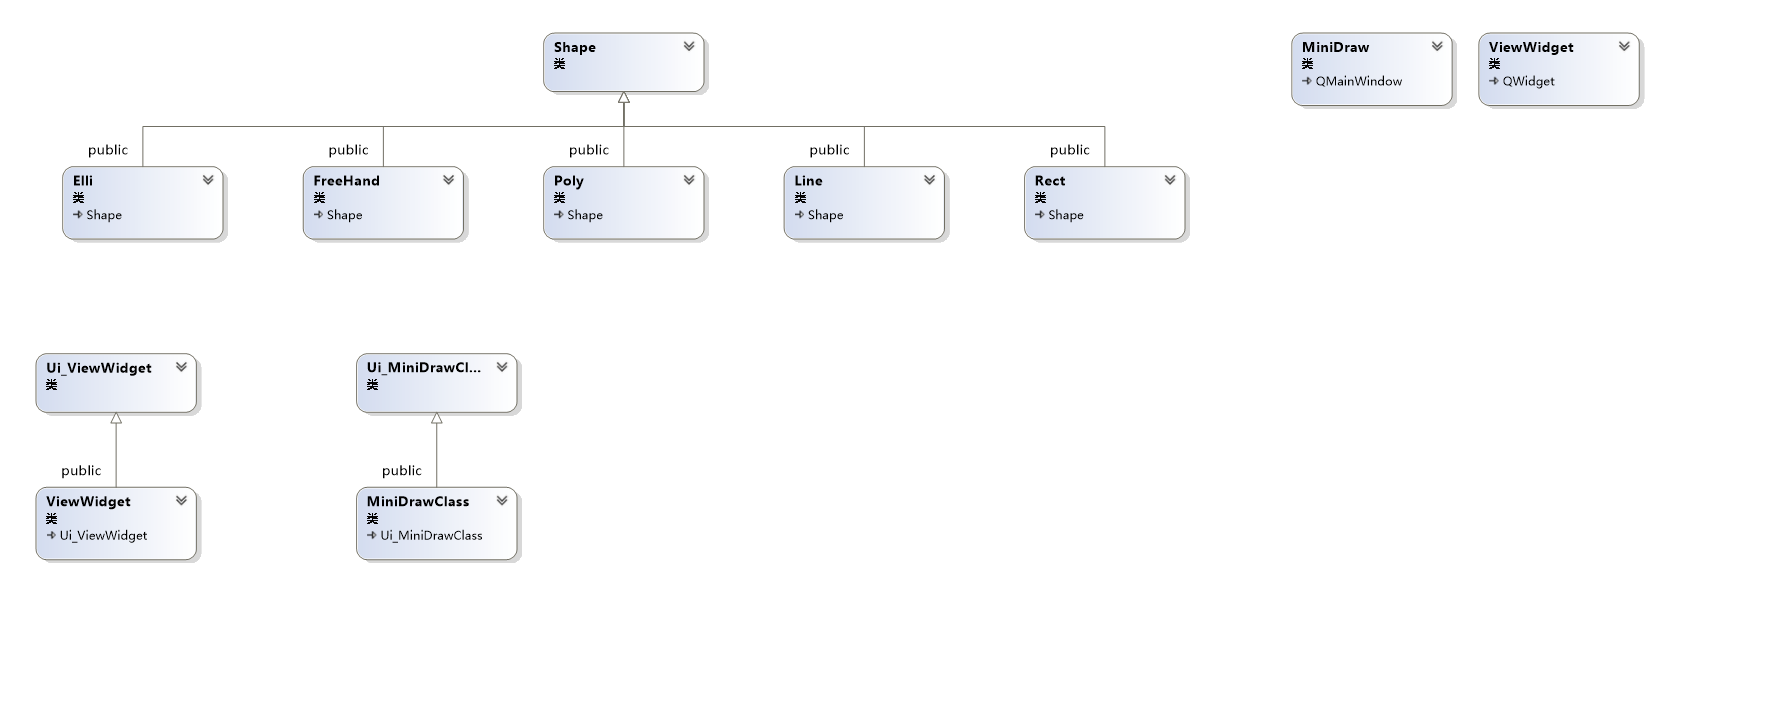
\includegraphics[width=18cm,height=10cm]{Class}
			
			\caption{项目的类视图} \label{Class.label}
		\end{center}
	\end{figure}

    两种方法分别用一个类来封装,并且这两个类都继承于父类warp。
    
    接下来我们描述一下需要实现的算法:
    
    输入:$n$对控制点$(p_i,q_i)$,$p_i=(x_i,y_i)$,$q_i=(x^{'}_i,y^{'}_i) \in \mathbb{R}^2$,其中$i=1,...,n$.其中$p_i$,$q_i$分别为起点和终点。
    
    目标:找到连续映射$f:\mathbb{R}^2 \rightarrow \mathbb{R}^2$,满足$f(p_i)=q_i$,$i=1,...,n$.
	
	\subsection{IDW算法}
	
	IDW算法的思路就是找到一个局部近似函数,保证起始点可以变换到终点。
	
	对原图中任一点P,变换后的点Q由下述的表达式给出
	$$ f(p)=\sum_{i=1}^nw_i(p)f_i(p) $$
	
	其中$w_i(p)$是权重函数,满足方程:
	$$	\left\{ 
	\begin{array}{lc}
		w_i(p_i) = 1 \\
		\sum_{i=1}^nw_i(p)= 1,\forall p\in \mathbb{R}^2  \\
		w_i(p) \geq 0, i=1,...,n \\
	\end{array}
	\right.$$
	
	DONALD SHEPARD提出了可以取权重函数为
	 $$ w_i(p)=\frac{\sigma_i(p)}{\sum_{j=1}^n \sigma_j(p)}$$
	 
	 其中$\sigma_j(p)=d(p,p_j)^{-\mu}$,在本实验中取$\mu = 2$。
	 
	 取局部近似函数$f_i$为线性函数,考虑$f_i(p)=q_i+(p-p_i)T_i$,并满足$T_i:\mathbb{R}^2 \rightarrow \mathbb{R}^2$,$T_i(0)=0$。
	 
	 通过解如下的最小二乘问题来确定$T_i$:
	 
	 $$min \sum_{j=1,j\ne i}^{n}\sigma_i(p_j) \left \| T_i(p_j-p_i)+q_i-q_j \right \|^2 $$
	
	
	\subsection{RBF算法}
	
	RBF算法是另一种思路的变换函数,它的取值仅依赖于点到标记点之间的距离。函数定义为如下形式:
	$$ f(p)=A(p)+T(p) $$
	$$T(p)=\sum_{i=1}^{n}\alpha_ig_i(d(p_i,p))$$
	其中 $$g_i(d)=(d^2+r^2)^{\frac{\mu}{2}}$$
	
	$\mu$可以取1或-1,本次实验默认取-1.$r$为$min_{j \ne i}d(p_i,p_j)$,系数$\alpha_i$可以通过解方程组$f(p_i)=q_i$解得。
	
	至此,需要处理的问题本质上已经转化为了解线性方程组。

	\subsection{填补白缝}
		由于在对图像进行变形的过程中存在对图像的拉伸,而处理的图形像素点是离散的,算法中构造的映射$f$不一定是一个满射,因此可能会出现无法填充到的点,也就是白缝。
	
	在实验中用周围非白缝的点来填充出现的白缝,即搜索3$\times$3内最近的点来填充。一开始我还打算取颜色RGB的均值来填充,后来经过对比发现并没有上面的这个方法好,于是作罢了。

	
	\section{结果展示}
	 \subsection{程序界面}
	
	   	\begin{figure}[H]
		\begin{center}
			
			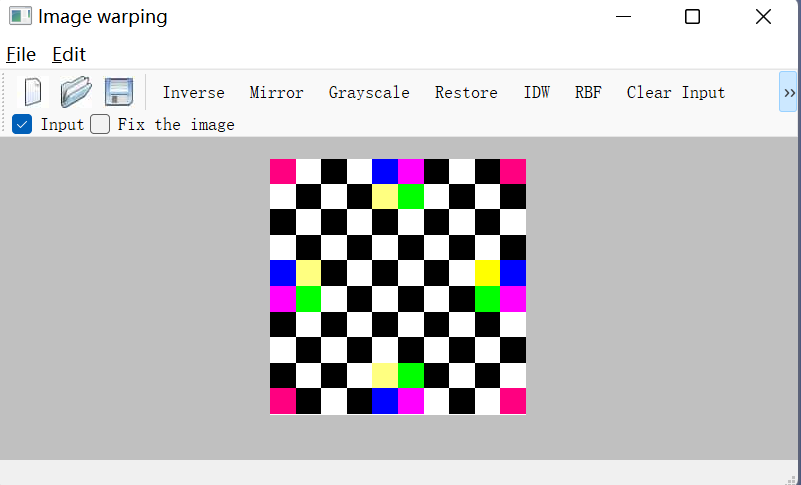
\includegraphics[width=11cm,height=6cm]{jiemian}
			
			\caption{程序界面} \label{jiemian.label}
		\end{center}
	\end{figure}

    程序界面如上所示
    
    \subsection{功能讲解}
    
    	\begin{itemize}
    	\item 最左边的图标是打开、保存图片
    \end{itemize}
    \begin{itemize}
    	\item Restore可以恢复图片原始的样子,Inverse,Mirror,Grayscale可以直接修改图片像素,具体可以看程序的说明。
    \end{itemize}
    \begin{itemize}
    	\item IDW,RBF在给定输入点的情况下会对图像做IDW,RBF变换
    \end{itemize}
    \begin{itemize}
    	\item 交互时,勾选Input,即可开始绘制输入点,蓝色代表起点,绿色代表终点。若要清除输入点,请点击Clear Input。取消勾选Input可以不显示输入的点,但已有的点还会保存(请注意)。
    \end{itemize}
    \begin{itemize}
    	\item 勾选Fix the image时,再用IDW、RBF时则会填补产生的白缝。使用时可以先不勾选,点击IDW/RBF,在Restore加载到原图,勾选上Fix在进行一次IDW/RBF。
    \end{itemize}
  
  
   \subsection{实验结果}
   
   注意:下面为了效果明显,都是固定四个边界点不动的
   
		\subsubsection{向外拉}
		
			\begin{figure}[H]
			\begin{center}
				
				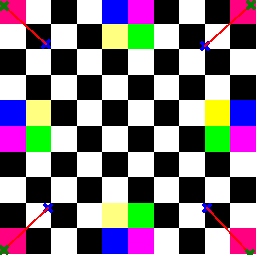
\includegraphics[width=4cm,height=4cm]{input1}
				
				\caption{控制点} \label{input2.label}
			\end{center}
		\end{figure}
	


\begin{table}[htbp]
	\centering
	\begin{tabular}{|c|c|c|}
		\hline
		\diagbox[width=3cm]{\textbf{使用方法}}{\textbf{是否填充}} & \textbf{是} & \textbf{否} \\
		\hline
		\multirow{2}{*}{\textbf{IDW}} & \raisebox{-0.5\height}{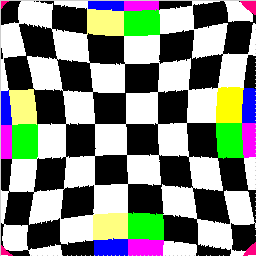
\includegraphics[width=4cm,height=4cm]{IDW wai.png}} & \raisebox{-0.5\height}{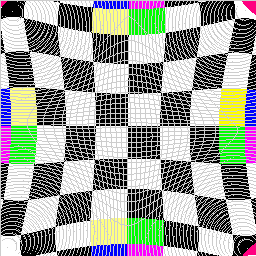
\includegraphics[width=4cm,height=4cm]{IDW wai bai.png}} \\
		\cline{2-3}
		& & \\
		\hline
		\multirow{2}{*}{\textbf{RBF}} & \raisebox{-0.5\height}{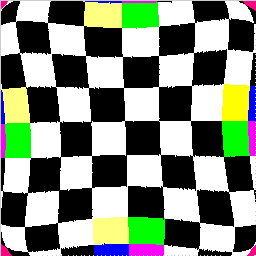
\includegraphics[width=4cm,height=4cm]{RBF wai.png}} & \raisebox{-0.5\height}{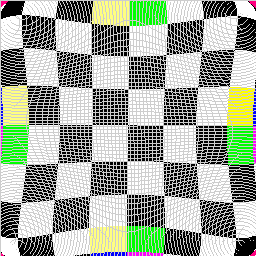
\includegraphics[width=4cm,height=4cm]{RBF wai bai.png}} \\
		\cline{2-3}
		& & \\
		\hline
	\end{tabular}
	\caption{向外拉的效果}
\end{table}


		\subsubsection{向内拉}
		
			\begin{figure}[H]
			\begin{center}
				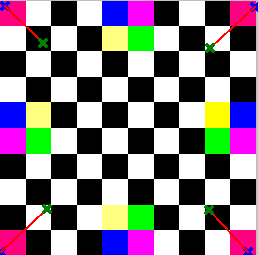
\includegraphics[width=4cm,height=4cm]{input2}
				\caption{控制点} 
			\end{center}
		\end{figure}
	
\begin{table}[htbp]
	\centering
	\begin{tabular}{|c|c|c|}
		\hline
		\diagbox[width=3cm]{\textbf{使用方法}}{\textbf{是否填充}} & \textbf{是} & \textbf{否} \\
		\hline
		\multirow{2}{*}{\textbf{IDW}} & \raisebox{-0.5\height}{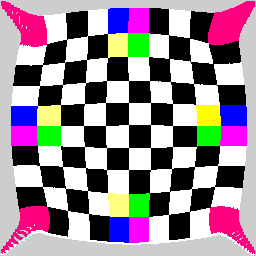
\includegraphics[width=4cm,height=4cm]{IDW nei.png}} & \raisebox{-0.5\height}{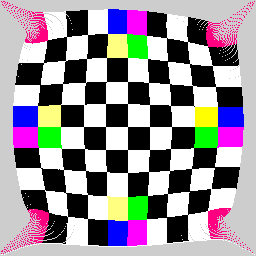
\includegraphics[width=4cm,height=4cm]{IDW nei bai.png}} \\
		\cline{2-3}
		& & \\
		\hline
		\multirow{2}{*}{\textbf{RBF}} & \raisebox{-0.5\height}{
\includegraphics[width=4cm,height=4cm]{RBF nei.png}} & \raisebox{-0.5\height}{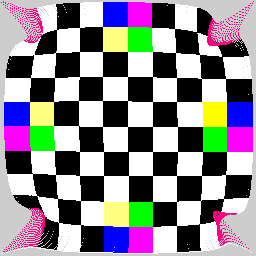
\includegraphics[width=4cm,height=4cm]{RBF nei bai.png}} \\
		\cline{2-3}
		& & \\
		\hline
	\end{tabular}
	\caption{向内拉的效果}
\end{table}
		
		
		\subsubsection{旋转变换}
	
		\begin{figure}[H]
		\begin{center}
			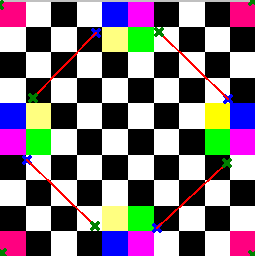
\includegraphics[width=4cm,height=4cm]{input3}
			\caption{控制点} 
		\end{center}
	\end{figure}
	
	\begin{table}[htbp]
		\centering
		\begin{tabular}{|c|c|c|}
			\hline
			\diagbox[width=3cm]{\textbf{使用方法}}{\textbf{是否填充}} & \textbf{是} & \textbf{否} \\
			\hline
			\multirow{2}{*}{\textbf{IDW}} & \raisebox{-0.5\height}{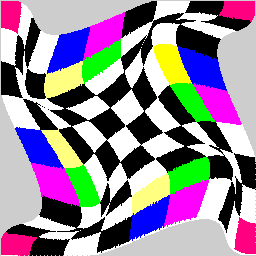
\includegraphics[width=4cm,height=4cm]{IDW ro.png}} & \raisebox{-0.5\height}{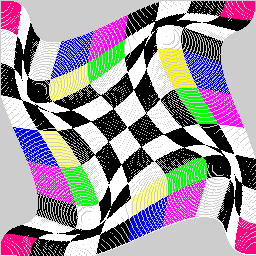
\includegraphics[width=4cm,height=4cm]{IDW ro bai.png}} \\
			\cline{2-3}
			& & \\
			\hline
			\multirow{2}{*}{\textbf{RBF}} & \raisebox{-0.5\height}{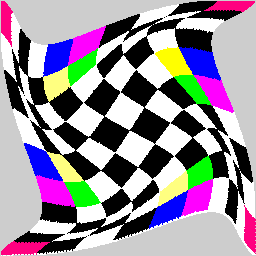
\includegraphics[width=4cm,height=4cm]{RBF ro.png}} & \raisebox{-0.5\height}{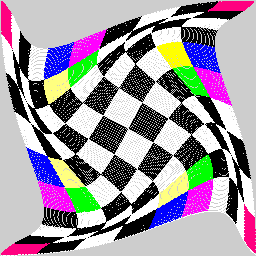
\includegraphics[width=4cm,height=4cm]{RBF ro bai.png}} \\
			\cline{2-3}
			& & \\
			\hline
		\end{tabular}
		\caption{旋转的效果}
	\end{table}

\subsubsection{其他例子}
	
		下面是一个处理蒙娜丽莎图像的测试数据(图6、图7):
	
	\begin{figure}
		\begin{minipage}[H]{0.5\linewidth}
			\centering
			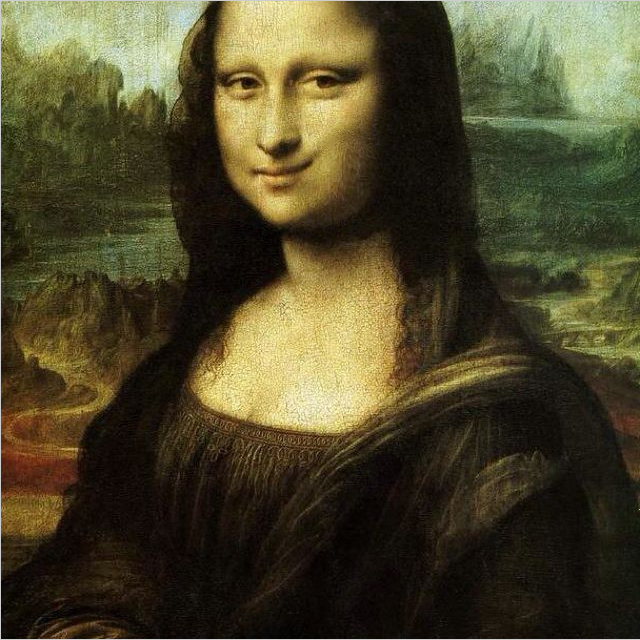
\includegraphics[scale=0.35]{art1.png}
			\caption{微笑}
		\end{minipage}%
		\begin{minipage}[H]{0.5\linewidth}
			\centering
			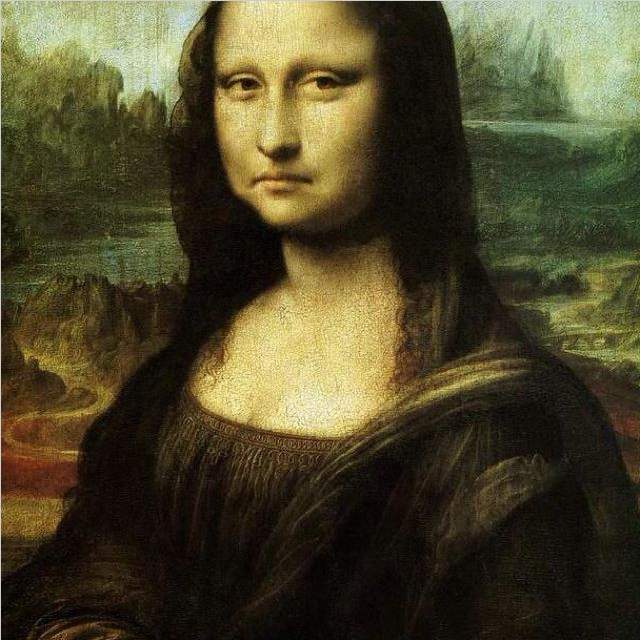
\includegraphics[scale=0.35]{art2.png}
			\caption{悲伤}
		\end{minipage}
	\end{figure}
	
	
	\section{总结与讨论}
	
	 \begin{itemize}
   \item	关于RBF和IDW的对比,直观上的感受是,RBF在收缩或拉伸时会更“好”一些,也就是会更加明显一点。比如同样拉伸,感觉RBF拉的距离会更远一点。
	 \end{itemize}
     \begin{itemize}
	\item	在性能上,能感受到IDW的性能是要差于RBF的。RBF运行速度快,复杂度也更低。不过时间原因,没有详细分析了。
	 \end{itemize}




	
	
	

	

\end{document}